\documentclass[12pt]{report}

% This is the Results section
\usepackage[margin=1.0in]{geometry}
\usepackage{graphicx}
\usepackage{textcomp} % Used for the < and > symbols in text mode, among others
\usepackage[superscript,biblabel,sort]{cite}
\usepackage[subrefformat=parens,labelformat=parens]{subfig}
\usepackage{caption}
\usepackage{gensymb}
\usepackage{longtable}
\usepackage{cleveref}
\usepackage{listings}

\bibliographystyle{aip}
\begin{document}
\chapter{Results and Discussion\label{results}}
\section{Validation of P and Q Matrices\label{results:PQValid}}
Comparison of the energy profiles calculated from the P and Q matrices with the copper energy profiles expected from the parameters defined in Bulatov \emph{et al.}'s code provides a way to validate the generated matrices.  \Cref{fig:compare100} shows the results from this comparison for the \textlangle{}100\textrangle{} set, with all six subsets shown in \Cref{appfig:compare100,appfig:compare110,appfig:compare111}.  The calculated energies match exactly the predicted values for all but a few points.  Each data set does not match the expected energy at 1\textdegree{}, and the tilt data sets also see this mismatch at their second to last data point.

\begin{figure}[ht!]
 \centering
 
 \subfloat[]{\label{fig:compare100Twist}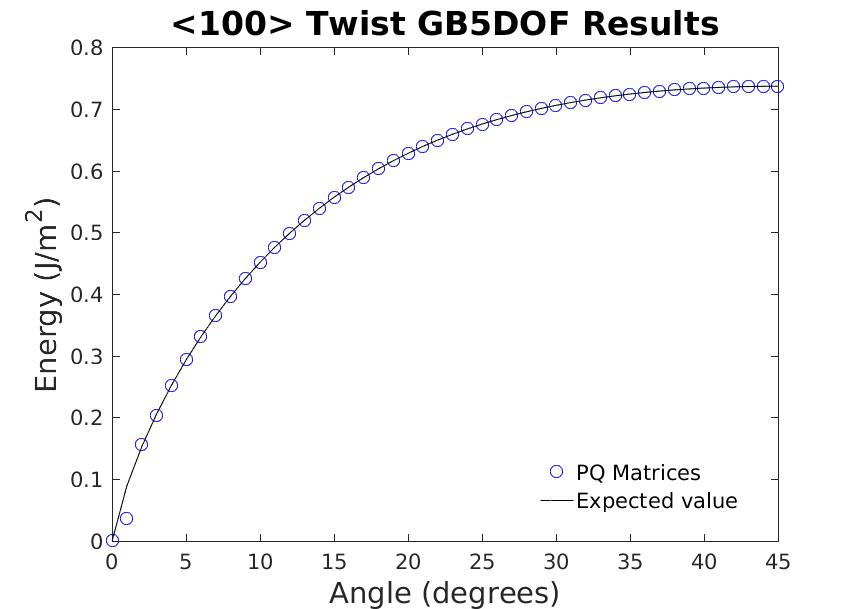
\includegraphics[scale=0.24]{Images/TestPQFit100Twist}}\quad
 \subfloat[]{\label{fig:compare100Tilt}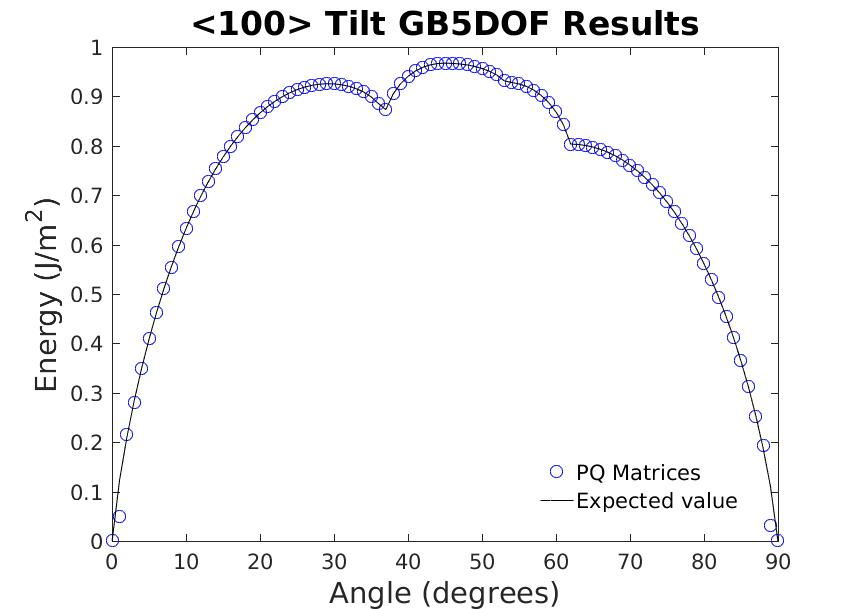
\includegraphics[scale=0.26]{Images/TestPQFit100Tilt}}
 \caption[A comparison of the \textlangle{}100\textrangle{} copper curve with the calculated results.]{\label{fig:compare100} The \textlangle{}100\textrangle{} twist \protect\subref{fig:compare100Twist} and tilt \protect\subref{fig:compare100Tilt} results for the P and Q matrices as compared to Bulatov \emph{et al.}'s energy profiles. Bulatov \emph{et al.}'s \lstinline!GB5DOF.m! MATLAB\textsuperscript{\textregistered} script calculated the expected values by using the default parameters.  The \lstinline!GB5DOF.m! script calculated the values using the generated matrices. With the exception of the data points at 1\textdegree{} in both \protect\subref{fig:compare100Twist} and \protect\subref{fig:compare100Tilt} and 89\textdegree{} in \protect\subref{fig:compare100Tilt}, the energies calculated from the matrices matches the expected curves exactly.}
\end{figure}

\section{Fitting Results\label{results:fit}}
\Cref{fig:100,fig:110,fig:111} compare the one-dimensional (1D) results from Harbison\cite{harbison2015} and this work.  The results show a general decrease in the grain boundary (GB) energies, allowing trends in the different subsets to emerge.  These trends allow for an all around better fit, but also introduce some unexpected results.  \Cref{app:params} shows the parameters calculated from the fitting procedure.

Initial MD recalculations of the \textlangle{}100\textrangle{} symmetric tilt GB energies using the 800 K anneal (\Cref{fig:100Tilt}) showed an unexpected deep cusp around 28\textdegree{}.  An analysis of the molecular dynamics (MD) simulation results for this misorientation revealed that, in this case, abnormally high pressures had caused the two crystals to realign.  This realignment caused the misorientation angle to change causing the GB energy to be much lower than expected.  Comparison with Harbison's simulation result revealed that the crystal structure from his simulation did not realign.  While Harbison's did not use annealed data and thus may not represent a global minimum, the data point follows the surrounding data's trend, justifying the use of his result.

Of the symmetric tilt GB energy sets, the \textlangle{}110\textrangle{} set has the most improvement.  All three sets showed a general decrease in the energy, increasing confidence in the accuracy of the fit for GB energies in uranium dioxide (UO\textsubscript{2}).  However, each of these sets provides more opportunity for research.  The \textlangle{}100\textrangle{} set needs more work done for data points after around 50\textdegree{}.  The scatter associated with those points seems to be higher, and the possibility of a slight cusp presents itself around 68\textdegree{}.  The \textlangle{}110\textrangle{} set as mentioned shows the most improvement, but some low points in the second and third ``humps" do not follow the trend, indicating further possibility for cusps.  The first part of the function (the first hump) needs additional data to determine the possibility of a cusp between 40\textdegree{} and 50\textdegree{}.  The fitted curve to the \textlangle{}111\textrangle{} set now has an unexpected upward trend.  The relatively high scatter associated with these data points leads to the possibility of a completely different set of functions to define this subset, meaning additional RSW functions would be required for example.

The twist GB energy sets vary in their success.  The \textlangle{}100\textrangle{} set shows little difference between Harbison's work and this work.  An unexpected slight positive concavity at the end of the fitting for this subset indicates the possibility of a cusp.  This cusp may occur around 30\textdegree{}.  The \textlangle{}110\textrangle{} set has a definite decrease in the overall energies, creating a plateau profile.  An additional cusp around 40\textdegree{} might improve the fit.  The \textlangle{}111\textrangle{} set has the least improvement.  Based on Bulatov \emph{et al.}'s work,\cite{bulatov2014} this work expected to see a plateau as Harbison's fitting demonstrated.\cite{harbison2015}  Instead, the fitting produced a curved energy profile, indicating the potential for at least one cusp, possibly around 35\textdegree{}.  Preliminary work has changed the number of parameters in an effort to maximize the quality of the fit with a minimal number of parameters. \Cref{fig:updatedGraphs} compares the current fitting to the tentative new fitting for three of the six 1D subsets.  These modified fits in general seem to fit better at the cost of additional parameters, with a smaller $\chi_{\textnormal{red}}^2$ value.  Still more parameters may be needed to accommodate additional cusps however.  A Levenberg-Marquardt MATLAB\textsuperscript{\textregistered} script calculated these tentative fits in part.\cite{gavin2016}

\Cref{fig:100PQ} shows the comparison between the values calculated from the P and Q matrices and the expected values from the MD calculations for the \textlangle{}100\textrangle{} subset.  \Cref{appfig:100PQ,appfig:110PQ,appfig:111PQ} shows all six subsets.  The \textlangle{}100\textrangle{} tilt subset has an unsolved scaling issue.  Overall, the results from the P and Q matrices match the fitted values, with a few anomalies needing to be addressed.

\begin{figure}[ht!]
 \centering
 
 \subfloat[]{\label{fig:100Twist}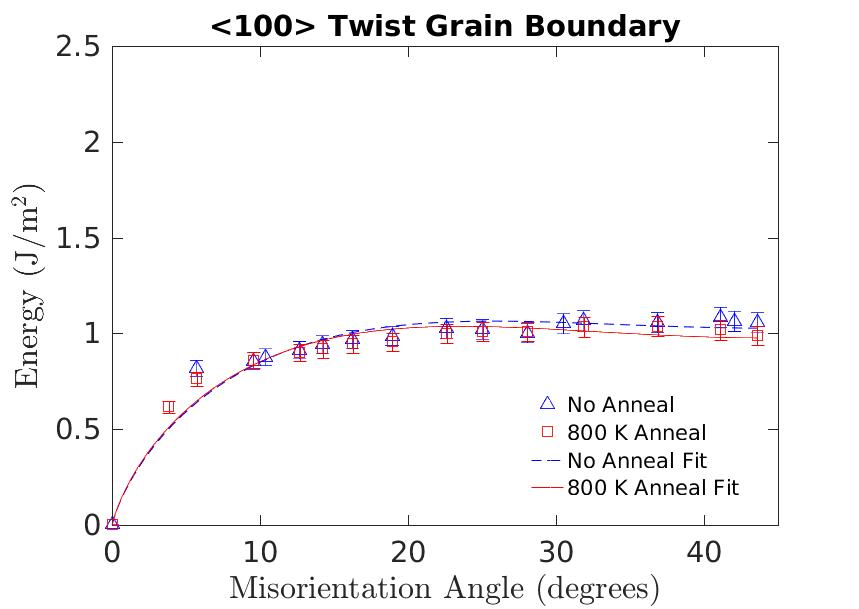
\includegraphics[scale=0.26]{Images/100TwistComparison}}\quad
 \subfloat[]{\label{fig:100Tilt}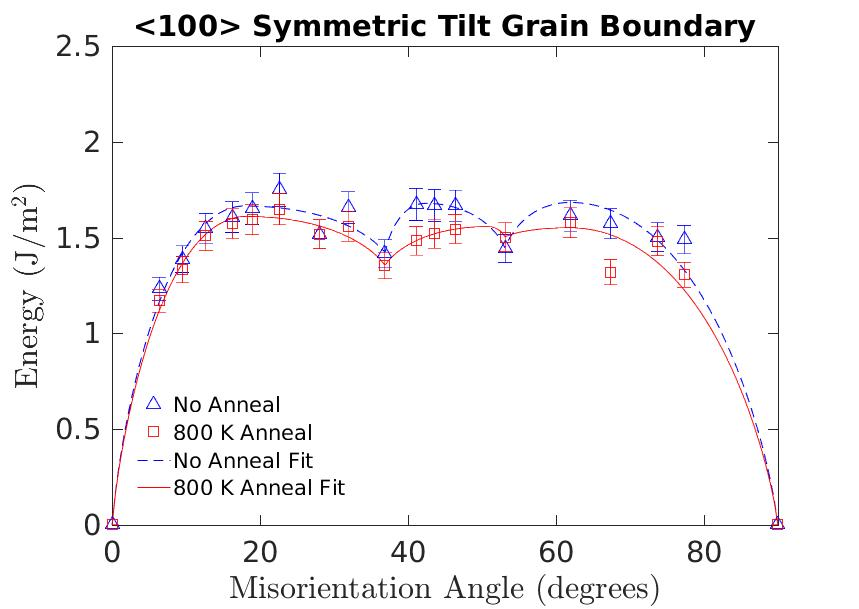
\includegraphics[scale=0.26]{Images/100SymmTiltComparison}}
 \caption[Results for the \textlangle{}100\textrangle{} fitting.]{\label{fig:100} The \textlangle{}100\textrangle{} twist \protect\subref{fig:100Twist} and tilt \protect\subref{fig:100Tilt} results.  In general the re-calculated energies are lower, with significant differences around 40\textdegree{} to 50\textdegree{} in the tilt subset.  The unexpected positive concavity in the twist subset around 40\textdegree{} may indicate the presence of a missing cusp.  Possible cusps exist around 30\textdegree{} in the twist subset, and around 68\textdegree{} in the tilt subset. }
 
\end{figure}

\begin{figure}[ht!]
 \centering
 
 \subfloat[]{\label{fig:110Twist}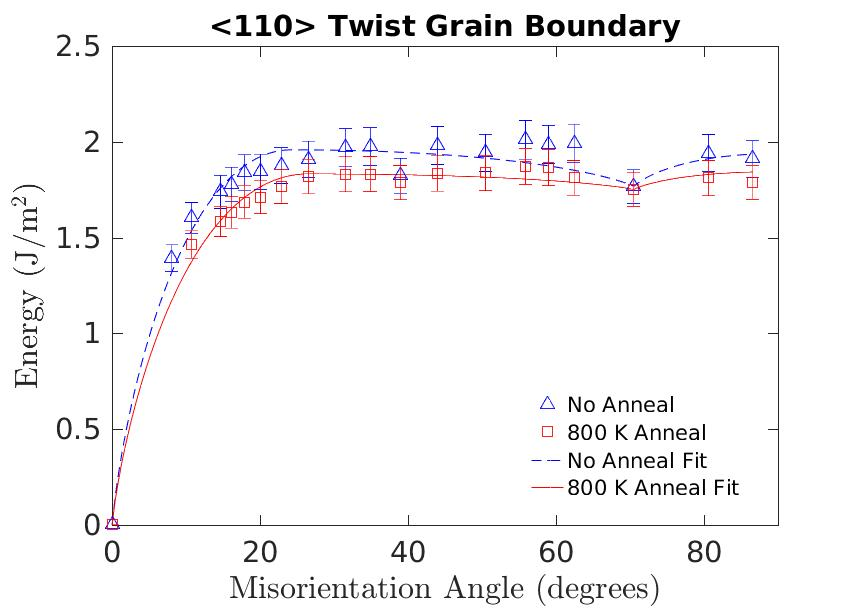
\includegraphics[scale=0.26]{Images/110TwistComparison}}\quad
 \subfloat[]{\label{fig:110Tilt}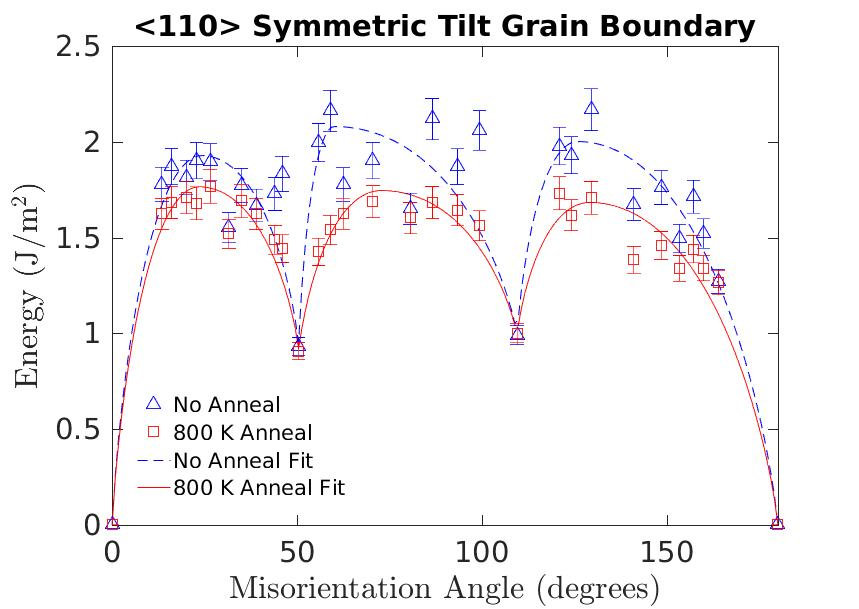
\includegraphics[scale=0.26]{Images/110SymmTiltComparison}}
 \caption[Results for the \textlangle{}110\textrangle{} fitting.]{\label{fig:110} The \textlangle{}110\textrangle{} twist \protect\subref{fig:110Twist} and tilt \protect\subref{fig:110Tilt} results.  Both subsets have significant decreases in energy.  The twist subset has a possible cusp at around 40\textdegree{}, and the tilt subset has possible cusps around 40\textdegree{}, 90\textdegree{}, and 140\textdegree{}.}
 
\end{figure}

\begin{figure}[ht!]
 \centering
 
 \subfloat[]{\label{fig:111Twist}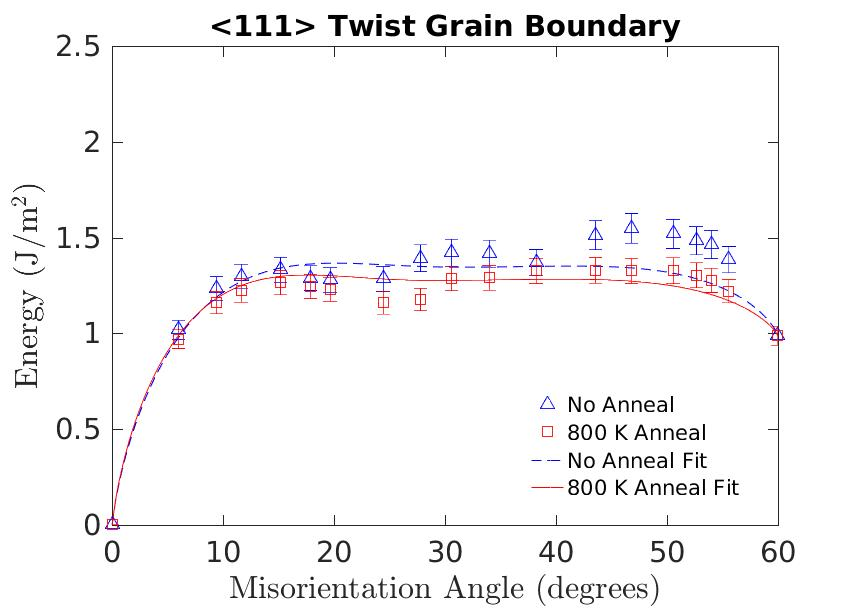
\includegraphics[scale=0.26]{Images/111TwistComparison}}\quad
 \subfloat[]{\label{fig:111Tilt}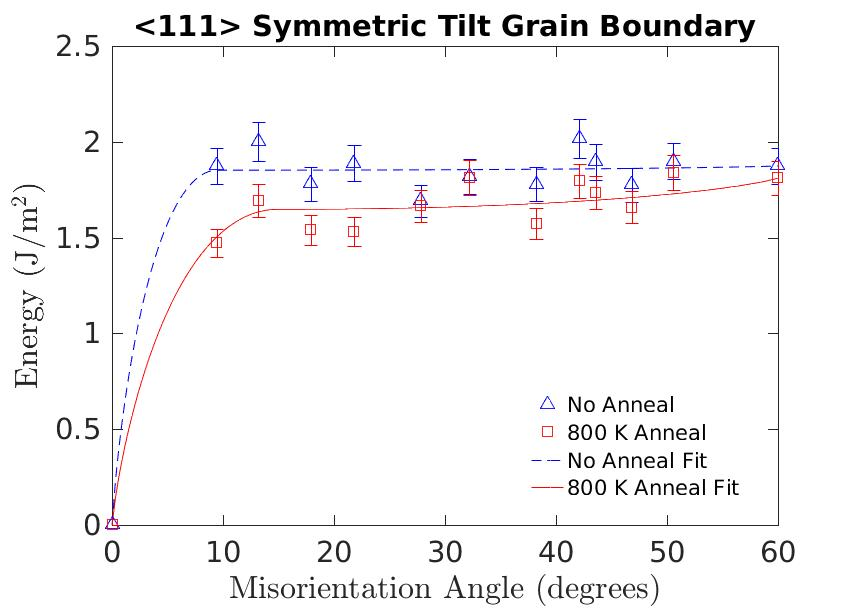
\includegraphics[scale=0.26]{Images/111SymmTiltComparison}}
 \caption[Results for the \textlangle{}111\textrangle{} fitting.]{\label{fig:111} The \textlangle{}111\textrangle{} twist \protect\subref{fig:111Twist} and tilt \protect\subref{fig:111Tilt} results.  Most energies are found to be lower, but some are found to be higher.  The unexpected positive concavity present in these results could indicate the presence of one or more cusps, with one possible location around 33\textdegree{}.  This work needs additional data to determine possible cusp locations for the tilt subset.}
 
\end{figure}

\begin{figure}[ht!]
 \centering
 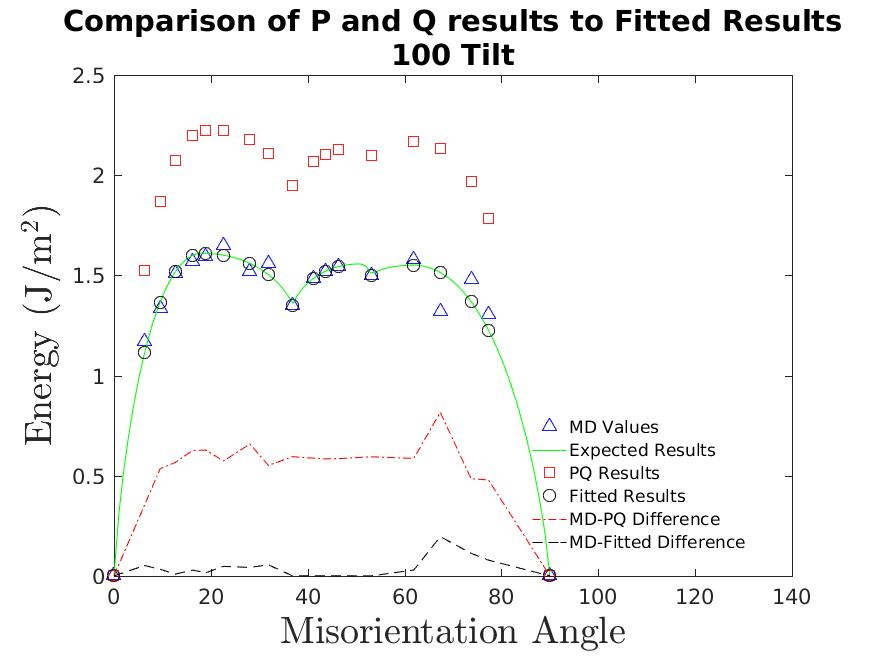
\includegraphics[scale=0.26]{Images/100TiltPQvsMD}
 \caption[Comparison of the PQ matrices with the expected result for \textlangle{}100\textrangle{} tilt.]{\label{fig:100PQ} A comparison of the expected value of the fitted function with the values calculated using the P and Q matrices for the \textlangle{}100\textrangle{} 1D tilt subset, with MD values shown for reference.  The cause of the scaling issue remains unknown.}
\end{figure}

\begin{figure}[ht!]
 
 \begin{minipage}{.5\linewidth}
 \centering
 \subfloat[]{\label{fig:updated100Twist}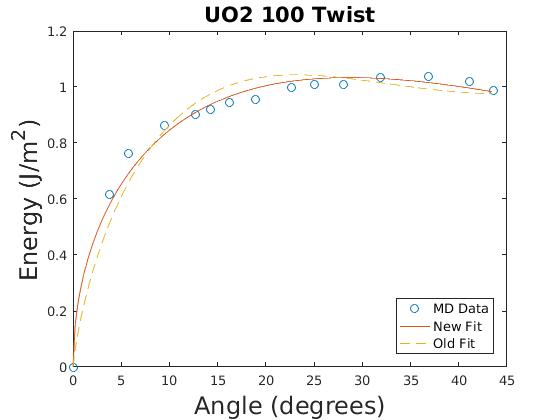
\includegraphics[scale=0.42]{Images/100Twist_marquardt}}
 \end{minipage}%
 \begin{minipage}{.5\linewidth}
 \centering
 \subfloat[]{\label{fig:updated110Twist}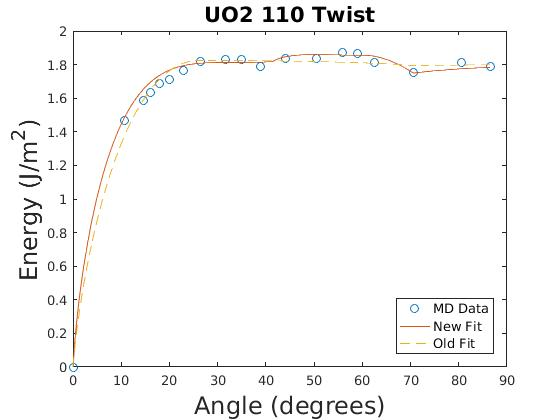
\includegraphics[scale=0.42]{Images/110Twist_vary_shaping_factor}}
 \end{minipage} \par\medskip
 \centering
 \subfloat[]{\label{fig:updated111Twist}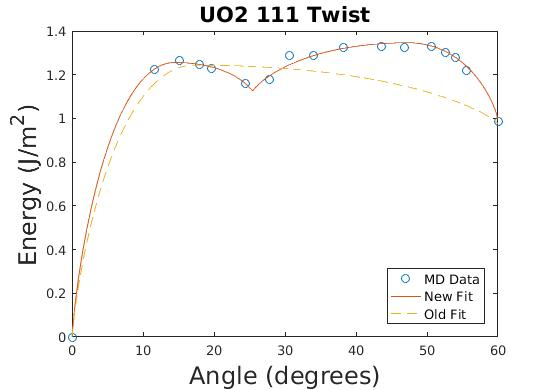
\includegraphics[scale=0.42]{Images/111Twist_marquardt}}
 
 \caption[Possible changes to fitting functions for the 1D twist subsets.]{\label{fig:updatedGraphs} A comparison of current fitting functions with a possible change to the functions.  Dashed lines show the original functions, and the solid lines show the updated functions, with MD results shown for reference. \protect\subref{fig:updated100Twist} shows a possible change from the Read-Shockley-Wolf (RSW) functions to a simple square root function multiplied by an exponential decay without any theoretical basis.  \protect\subref{fig:updated110Twist} attempts to fit to a cusp around 40\textdegree{}.  Further work can be done to find a better fit for this subset. \protect\subref{fig:updated111Twist} shows the most potential improvement.  The potential fit increases the total number of parameters by three to fit to the cusp around 28\textdegree.  A quick glance at the MD values compared to the fit shows a great improvement from the current fit.  To create the graph shown in \protect\subref{fig:updated111Twist} this work spliced two additional RSW functions into the original function.  This created a total of four RSW functions for this subset.}
 
\end{figure}

\section{Reduced Chi-square Results\label{results:chi2red}}
The $\chi_{\textnormal{red}}^2$ values are much smaller than one for every data set regardless of the method used to calculate the statistic, with the exception of the \textlangle{}100\textrangle{} symmetric tilt subset using the P and Q matrices.  This subset has a high $\chi_{\textnormal{red}}^2$ value due to the scaling issue.  Because of the low $\chi_{\textnormal{red}}^2$ values, the fitted functions overfit the data.\cite{bevington2003}  \Cref{table:chi2} lists the $\chi_{\textnormal{red}}^2$ values for the 1D subsets using the two different methods for calculation. 

\begin{table}[ht!]
\centering
\caption{A list of the $\chi_{\textnormal{red}}^2$ results using two different methods: using the P and Q matrices for the various orientations to test the fit, and comparing the results of the 1D fits to the 1D data.  The values for $\chi_{\textnormal{red}}^2$ are all less than one with the exception of the \textlangle{}100\textrangle{} symmetric tilt using the P and Q matrices.  These values indicate an over-fit to the data.}
\label{table:chi2}
\begin{tabular}{{l c c c c}}
1D Subset & \multicolumn{2}{c}{$\chi_{\textnormal{red}}^2$ using P and Q matrices} & \multicolumn{2}{c}{$\chi_{\textnormal{red}}^2$ comparing the 1D fits} \\[5pt]
          & No Anneal & 800 K Anneal & No Anneal & 800 K Anneal \\
\hline
\textlangle{}100\textrangle{} Twist & 0.0953 & 0.1074 & 0.0752 & 0.0722 \\
\textlangle{}110\textrangle{} Twist & 0.1010 & 0.1874 & 0.0400 & 0.0137 \\
\textlangle{}111\textrangle{} Twist & 0.3041 & 0.1139 & 0.4966 & 0.1516 \\
\textlangle{}100\textrangle{} Tilt & 0.1038 & 8.7702 & 0.0846 & 0.0932 \\
\textlangle{}110\textrangle{} Tilt & 4.9799 & 0.3277 & 0.5951 & 0.1762 \\
\textlangle{}111\textrangle{} Tilt & 0.1566 & 0.7814 & 0.1315 & 0.1355 \\
\hline
Overall $\chi_{\textnormal{red}}^2$ & 1.7652 & 1.4893 & 0.2678 & 0.1153 \\
\end{tabular}
\end{table}

\clearpage
\bibliography{gbCharacter}

\end{document}
